\documentclass[9pt]{developercv} % Default font size, values from 8-12pt are recommended
\begin{document}

\begin{minipage}[t]{0.45\textwidth} % 45% of the page width for name
	\vspace{-\baselineskip} % Required for vertically aligning minipages
	
	\colorbox{black}{{\HUGE\textcolor{white}{\textbf{\MakeUppercase{BOB BASS}}}}} % First name
	
	\vspace{6pt}
	
	{\huge MMTMM} % Career or current job title
\end{minipage}
\begin{minipage}[t]{0.275\textwidth} % 27.5% of the page width for the second row of icons
	\vspace{-\baselineskip} % Required for vertically aligning minipages
	\icon{Github}{12}{\href{https://github.com/machine-hum/mmtmm}{github.com/machine-hum/mmtmm}}\\
\end{minipage}

\vspace{0.5cm}

\cvsect{Who Am I?}

\begin{minipage}[t]{0.4\textwidth} % 40% of the page width for the introduction text
	\vspace{-\baselineskip} % Required for vertically aligning minipages
	
The BOB BASS is a 100\% open source drum modules inspired from the 808 Bass drum. It features the same drum core as the 808 and various other features, such as filters, tuning and an \textcolor{red}{overdrive}.

\end{minipage}

\hfill % Whitespace between

\cvsect{Getting Started}

The BOB BASS requires power. Then post a picture, then outline what all the knobs do and what to plug into.


\begin{center}
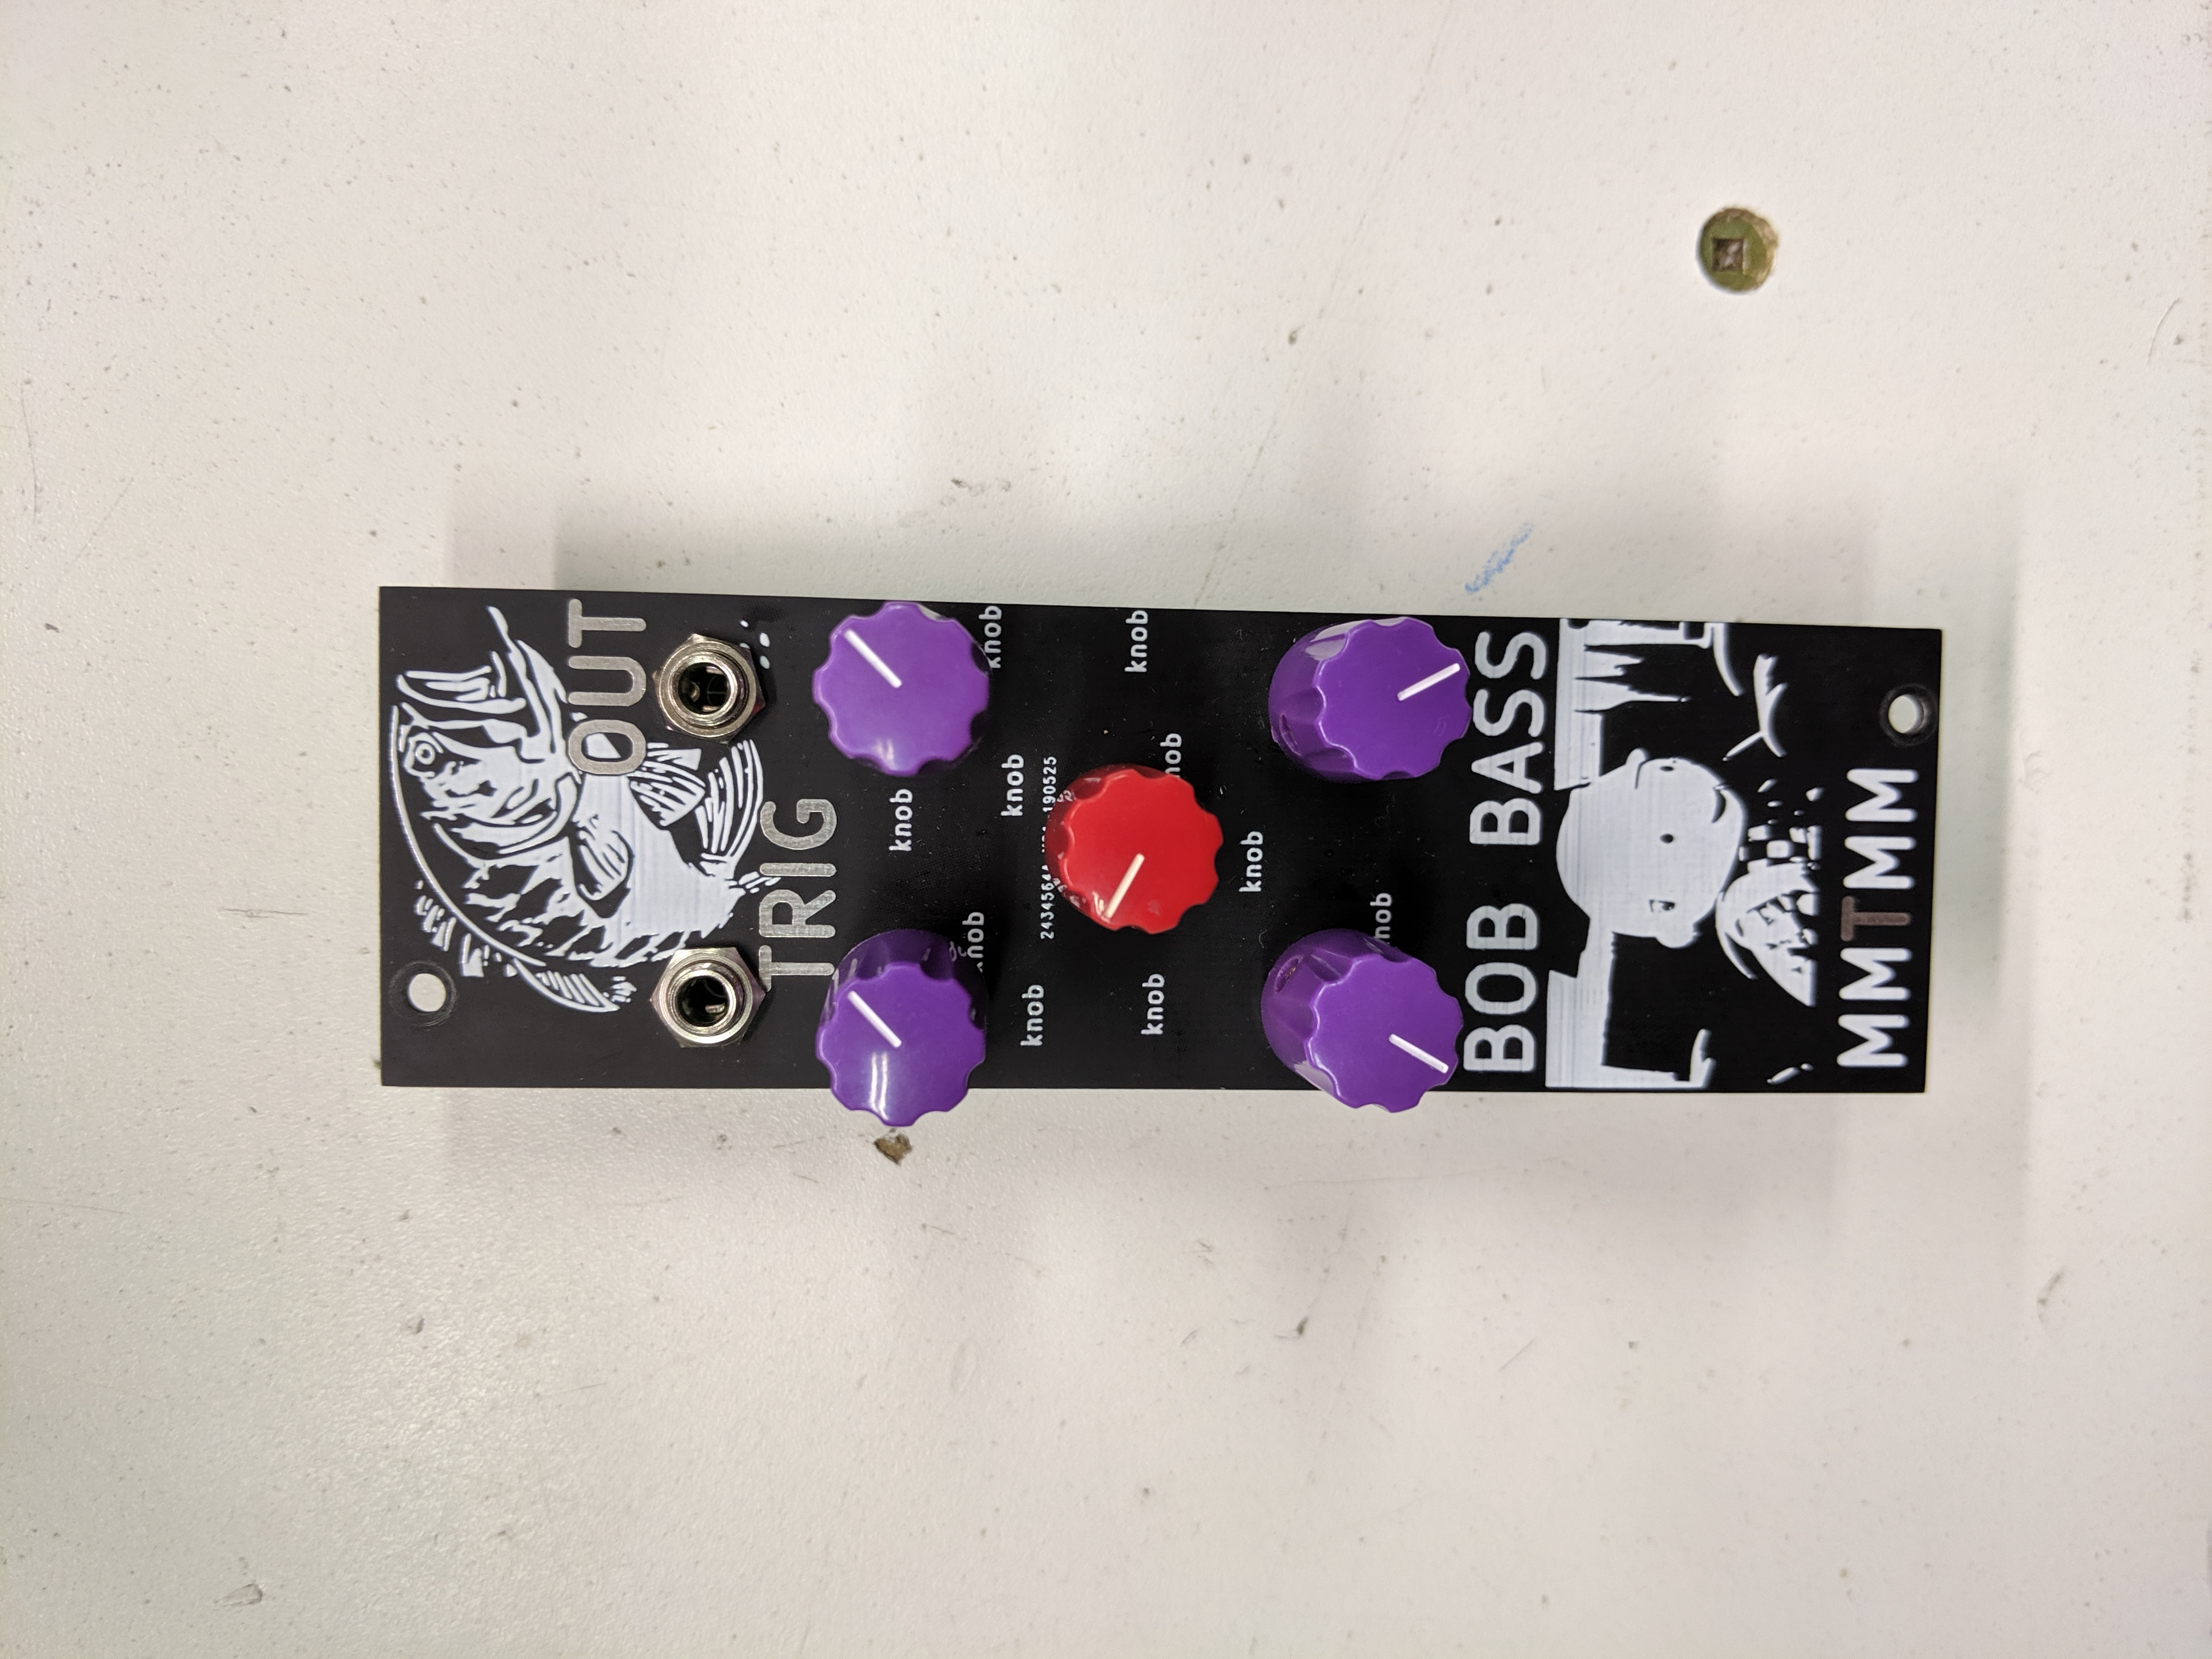
\includegraphics[scale=0.12,angle=-90,trim={20cm 30cm 15cm 30cm},clip]{../images/IMG_20190725_210209.jpg}
\end{center}

\cvsect{Schematic}
\begin{center}
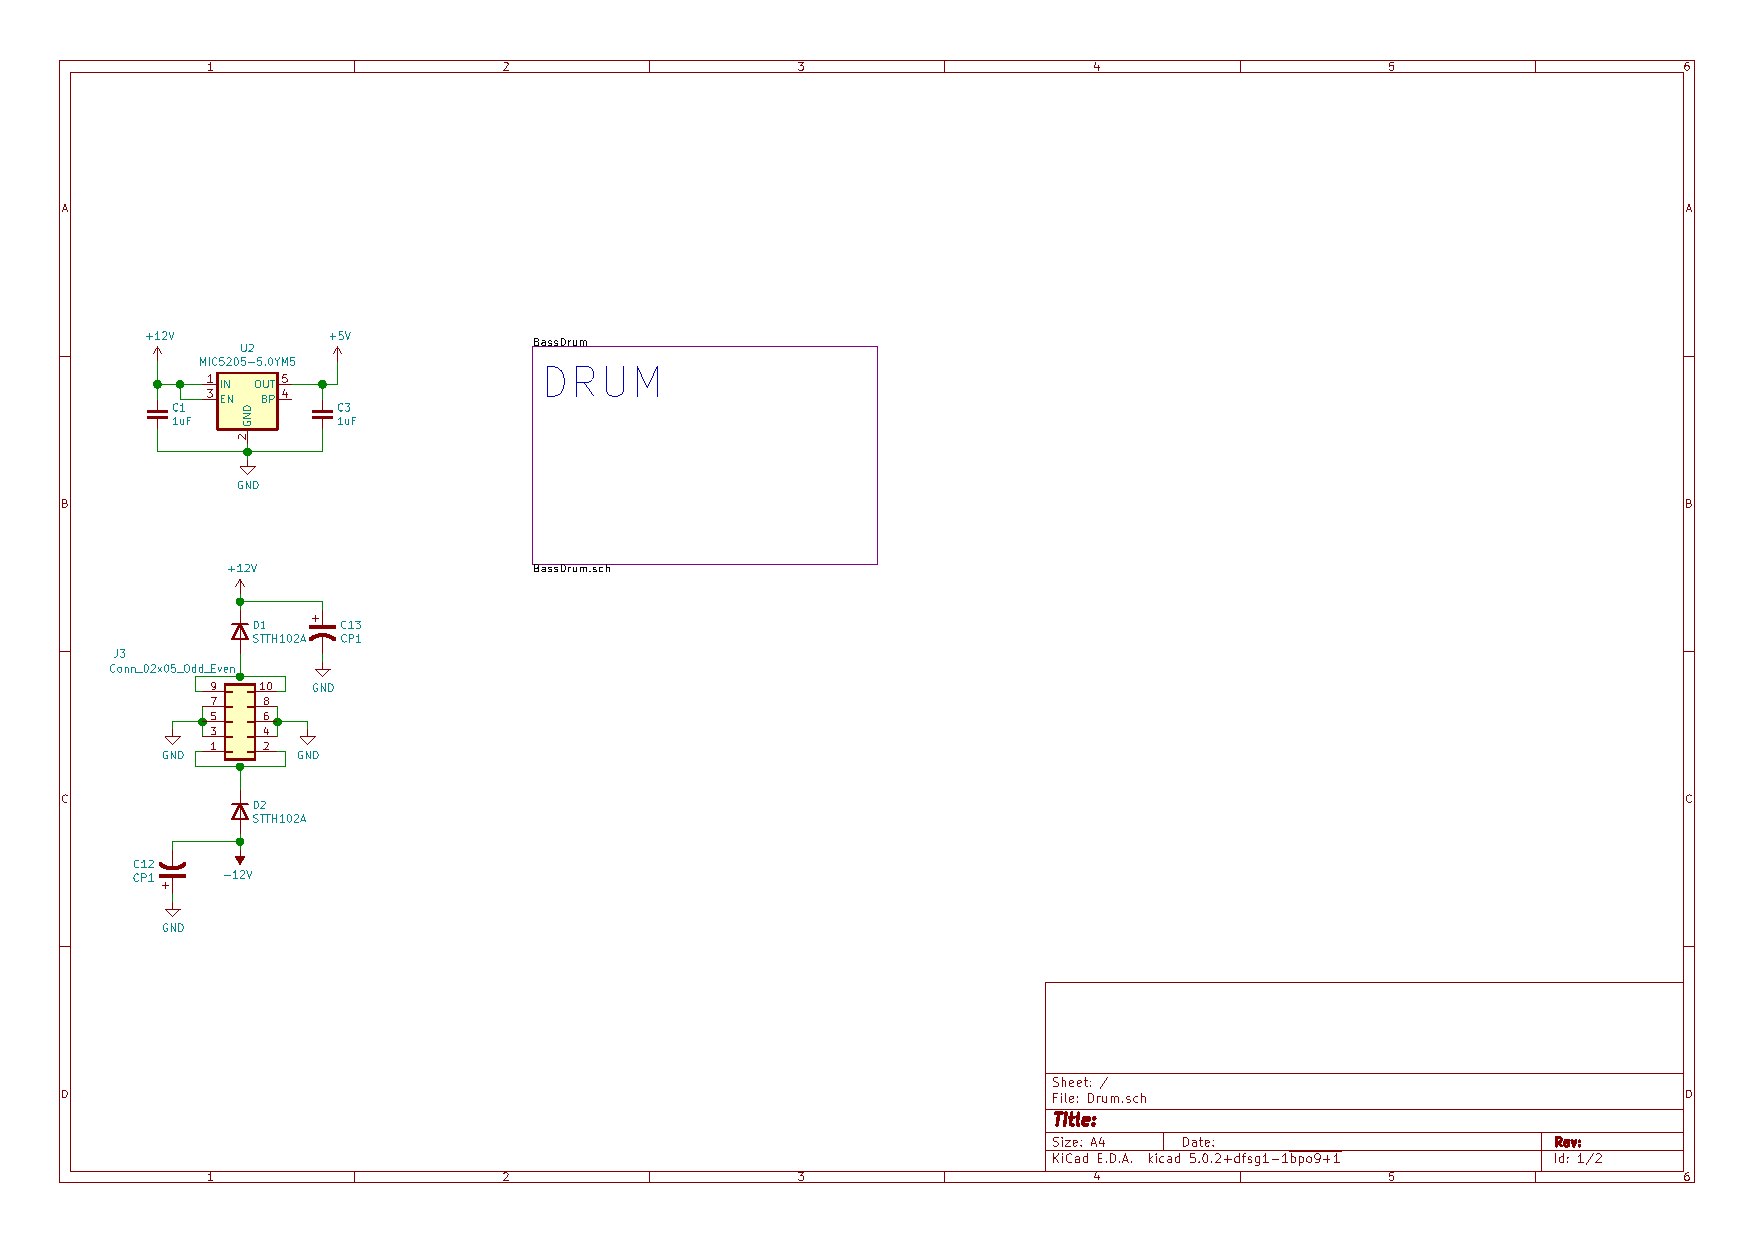
\includegraphics[page=1,scale=0.6]{../Drum/plot/Drum.pdf}
\end{center}

\\

\begin{center}
\includegraphics[page=2,scale=0.6]{../Drum/plot/Drum.pdf}
\end{center}

\cvsect{Transfer Function for Drum Core}

Equation \ref{tfd} is the transfer function for the drum, while Equation \ref{tfn} is the standard form.
\begin{equation}
G(s) = \frac{\frac{-s}{R_7C_1}}{s^2 + \frac{s}{R_6}(\frac{1}{C_1} + \frac{1}{C_2}) + \frac{1}{R_6R_7C_1C_2}}
\label{tfd}
\end{equation}

\begin{equation}
G(s) = \frac{k\cdot w_n^2}{s^2 + 2\zeta w_n s + w_n^2}
\label{tfn}
\end{equation}

\begin{equation}
w_n = \frac{1}{\sqrt{R_6R_7C_1C_2}}
\end{equation}

This forumula came from the internet... Figure out how to get it from the TF.

\begin{equation}
\zeta = \frac{\sqrt{\frac{C_1}{C_2}} + \sqrt{\frac{C_2}{C_1}}}{\sqrt{\frac{R_6}{R_7}}}
\end{equation}

\end{document}
